\documentclass[tikz]{standalone}
\usepackage{tikz}
\usetikzlibrary{bayesnet}
\begin{document}

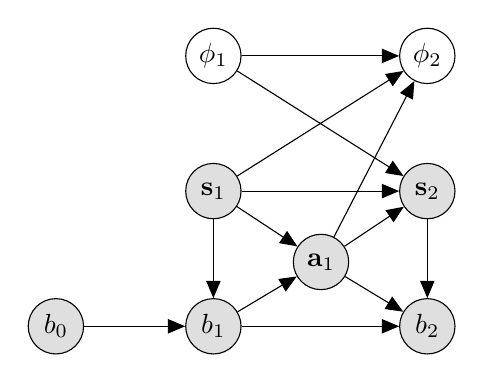
\begin{tikzpicture}[node distance=2cm]
  % Define nodes
  \node[obs]                                               (s1)  {$\mathbf{s}_1$};
  \node[latent, above=of s1]                               (phi1){$\phi_1$};
  \node[latent, right=2cm of phi1]                         (phi2){$\phi_2$};
  \node[obs,    right=of s1, xshift=-0.35cm, yshift=-0.9cm] (a1)  {$\mathbf{a}_1$};
  \node[obs,    below=of s1, xshift=-2cm]                  (b0)  {$b_0$};
  \node[obs,    below=of s1]                               (b1)  {$b_1$};
  \node[obs,    right=2cm of s1]                           (s2)  {$\mathbf{s}_2$};
%  \node[obs,    right=of s2, xshift=0.15cm, yshift=-0.9cm] (a2)  {$\mathbf{a}_2$};
  \node[obs,    below=of s2]                               (b2)  {$b_2$};

  % Connect the nodes
  \edge {s1,b1}      {a1};
%  \edge {s2,b2}      {a2};
  \edge {phi1,s1,a1} {s2};
  \edge {b0,s1}      {b1};
  \edge {b1,a1,s2}   {b2};
  \edge {phi1,s1,a1} {phi2};
\end{tikzpicture}

\end{document}